\documentclass[a4paper,12pt, oneside]{article}

\title{\textbf{Elaborato per il corso Basi di dati} \\ \large A.A 2023/2024 \\ Progetto di una base di dati per la vendita di pizze}
\author{Gabos Norbert \\ 0000970451 \\ tiberiunorbert.gabos@studio.unibo.it }
\date{}

\usepackage[T1]{fontenc}
\usepackage[utf8]{inputenc}
\usepackage[italian]{babel}
\pagestyle{plain}
\usepackage{graphicx}
\graphicspath{{images/}}

\begin{document}

\maketitle

\newpage
\tableofcontents{}
\newpage

\section{Analisi dei requisiti}

Si vuole realizzare un database per la gestione automatica della vendita
delle pizze. Pertanto la base di dati dovrà immagazzinare i dati e gli
clienti dei loro ordini, nonché dare la possibilità al venditore di
inserire o modificare le proprie pizze.

\subsection{Intervista}

Si intende gestire la clientela del negozio registrando il nome, il
cognome, l'email, il numero di telefono e l'indirizzo di ogni individuo. Ogni
cliente deve essere in grado di effettuare il proprio ordine, con un
limite massimo di 10 pizze. Si possono avere al massimo 4 ordini ogni
quarto d'ora, al fine di garantire la consegna degli ordini nelle
fasce orarie successive in modo puntuale.
Inoltre il cliente potrà scegliere se farsi recapitare a casa proprie
le pizze, oppure se le vuole venire a prendere lui, nel primo caso
bisogna chiedere all'utente l'indirizzo a cui recapitare le pizze.

Si vuole tener traccia dello storico degli ordini di ciascun utente in
modo da garantire al proprietario di effettuare delle stime sui propri
prodotti. Gli utenti devono anche poter visualizzare tutti i propri
ordini e avere la possibilità di modificare o cancellare il proprio
account. In caso di cancellazione dell'account di un cliente si devono
anche cancellare tutte le operazione che esso ha effettuato, come i
propri ordini o eventuali future funzioni. Ciò serve per garantire la
privacy degli individui.

Ciascuna pizza deve appartenere a una categoria, tra cui "Pizze
classiche", "Pizze speciali" e "Impasto napoletano". Ogni pizza è
caratterizzata da un prezzo, un nome e una lista di ingredienti e
allergeni, come latticini, noci, uova, ecc.

Infine, è necessario tenere traccia dei pizzaioli, che devono essere
in grado di modificare le pizze e gli ingredienti, cancellare quelli
esistenti o aggiungerne di nuovi.

Possono anche consultare il portale per visualizzare la classifica delle
pizze più vendute e meno vendute. Ciò server per apportare modifiche
al menu alla fine dell'anno, come la modifica, oppure la cancellazione
di alcune pizze.

\newpage
\begin{figure}[h]
    \centering
    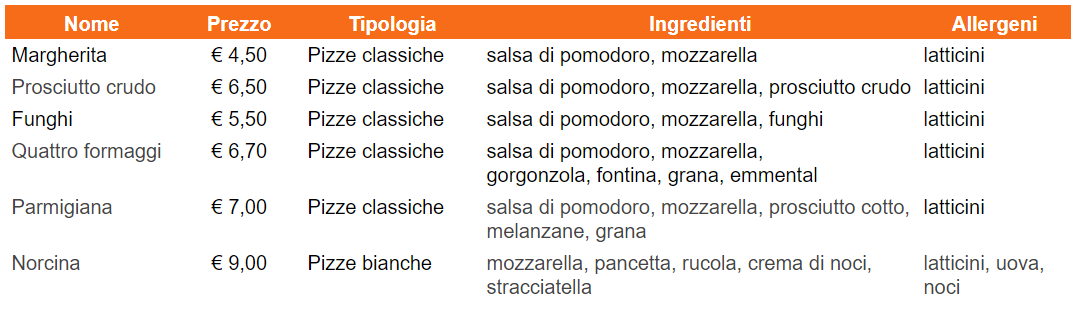
\includegraphics[width=1\textwidth]{esempio_pizze.png}
    \caption{Esempio dell'elenco di pizze.}
    \label{fig:esempio_pizze}
\end{figure}

\subsection{Estrazione dei concetti principali}

Dopo aver esaminato e compreso i requisiti, si procede con la redazione
di un testo che sintetizza tutti i concetti, concentrandosi in
particolare sull'estrazione dei principali e sulla rimozione delle
ambiguità individuate in precedenza.
\begin{quote}

Per ciascun cliente, è necessario registrare il proprio nome, cognome,
numero di telefono, indirizzo email e un identificativo univoco assegnato
al momento della creazione dell'account. Ogni cliente avrà accesso a un
listino completo delle pizze e potrà selezionare quelle desiderate per
aggiungerle al proprio ordine. Inoltre, l'applicazione gestirà
completamente la funzione del carrello, salvando eventuali modifiche
sul dispositivo dell'utente.

Gli ordini saranno catalogati in intervalli di quindici minuti,
dall'orario di apertura a quello di chiusura, con limitazioni sia
sul numero complessivo di ordini che sul numero di pizze per ogni
ordine. Gli ordini possono essere di due tipi: consegna a domicilio o
ritiro dell'ordine, nel primo caso bisogna anche memorizzare l'indirizzo
di recapito. Ogni utente potrà visualizzare la propria cronologia degli
ordini, ma solo il proprietario avrà accesso a tutti gli ordini
effettuati.

Per ogni pizza, è necessario memorizzare il nome come identificatore
unico, il tipo, gli ingredienti, gli allergeni e il prezzo.

Il proprietario avrà la capacità di visualizzare e modificare tutte
le informazioni relative a ciascuna pizza. Infine, avrà la possibilità
di consultare una classifica contenente le 5 pizze più vendute e meno
vendute.
\end{quote}

Elenco delle principali azioni richieste:
\begin{enumerate}
    \item Inserimento di un nuovo cliente
    \item Eliminazione di un cliente
    \item Inserimento di un socio
    \item Creazione di un ordine
    \item Eliminazione di una pizza
    \item Modifica delle caratteristiche di una pizza
    \item Aggiunta di ingredienti nuovi
    \item Eliminazione di un ingrediente
    \item Visualizzazione delle pizze con relativi dettagli
    \item Visualizzazione degli ordini dei relativi clienti
    \item Visualizzazione della classifica delle pizze più e meno vendute
\end{enumerate}

\section{Progettazione Concettuale}
\subsection{Schema scheletro}

Per l'entità \textbf{Cliente}, si è deciso di modellarla come
generalizzazione, assieme a \textbf{Proprietario}, di \textbf{Utente}.

Dall'analisi del dominio si evince che solo un numero limitato di ordini
più essere effettuato in una certa fascia oraria, per ciò è stata creata
l'entità \textbf{Fascia oraria} e \textbf{Ordine}, con un limite di 4
istanze per fascia oraria. Inoltre l'entità \textbf{Ordine} è identificata
da una data, dalla fascia oraria e dall'id del cliente, cosi si evita che
un cliente possa effettuare ordini multipli saturando il limite imposto.

\subsection{Schema finale}

\section{Progettazione Logica}
\subsection{Stima del volume dei dati}
\subsection{Descrizione delle operazioni principali e stima della loro frequenza}
\subsection{Schemi di navigazioni e tabelle degli accessi}
\subsection{Raffinamento dello schema}
\subsection{Analisi delle ridondanze}
\subsection{Traduzione di entità e associazioni in relazioni}
\subsection{Schema relazionale finale}
\subsection{Traduzione delle operazioni in query SQL}

\section{Progettazione dell'applicazione}
\subsection{Descrizione dell'architettura dell'applicazione realizzata}

\end{document}
